% ======================================================================
% fig_trap -- standalone build of a figure that main.tex also draws inline.
% ----------------------------------------------------------------------
% The tikzpicture below is copied VERBATIM from main.tex, so this file and
% the inline version render identically. Build with:
%     pdflatex fig_trap.tex
% The standalone class crops the PDF to the picture's bounding box, so no
% trim/clip is ever needed in the paper.
%
% Fonts: the picture inherits times/helvet, so every glyph is Type 1 and
% embedded by pdflatex. Nothing is rasterised, so DPI does not apply.
% ======================================================================
\documentclass[border=2pt]{standalone}

\usepackage{times}
\usepackage{helvet}
\usepackage{courier}
\usepackage{amsmath}
\usepackage{amssymb}
\usepackage{xcolor}
\usepackage{pifont}
\usepackage{tikz}
\usetikzlibrary{arrows.meta,positioning}

%% ======================================================================
%% preamble-figures.tex
%% ----------------------------------------------------------------------
%% Every definition the figures need, kept identical to main.tex's preamble.
%% Shared by the standalone builds in this folder; main.tex carries its own
%% copy so that the submitted source stays a single .tex file.
%% ======================================================================

\providecommand{\method}{\textsc{ESV}}

%% --- comparison-table glyphs (fig_trap uses \yes / \no) ---------------
\definecolor{okgreen}{RGB}{0,122,87}
\definecolor{okred}{RGB}{176,42,32}
\providecommand{\yes}{\textcolor{okgreen}{\ding{51}}}
\providecommand{\no}{\textcolor{okred}{\ding{55}}}
\providecommand{\na}{\textcolor{black!45}{--}}

%% --- figure fills, shaded by what each step costs ---------------------
\definecolor{cshared}{RGB}{226,226,226}
\definecolor{ccode}{RGB}{205,228,243}
\definecolor{ccall}{RGB}{252,230,192}
\definecolor{ccallb}{RGB}{191,118,0}
\definecolor{cout}{RGB}{206,238,227}
\definecolor{ctrap}{RGB}{250,222,218}

%% --- plot colours and markers -----------------------------------------
%% Marker shapes are core TikZ nodes, so every glyph is vector and uses the
%% document's Type 1 text fonts: no Type 3 subsets, no raster, nothing to crop.
\definecolor{pblue}{RGB}{31,97,160}
\definecolor{pgreen}{RGB}{0,122,87}
\definecolor{pgrey}{RGB}{95,95,95}
\providecommand{\mkopensq}[2]{\node[draw=#2,fill=white,line width=.6pt,rectangle,inner sep=1.5pt] at #1 {};}
\providecommand{\mkfillsq}[2]{\node[draw=#2,fill=#2,rectangle,inner sep=1.5pt] at #1 {};}
\providecommand{\mkopenci}[2]{\node[draw=#2,fill=white,line width=.6pt,circle,inner sep=1.5pt] at #1 {};}
\providecommand{\mkfillci}[2]{\node[draw=#2,fill=#2,circle,inner sep=1.5pt] at #1 {};}
%% #1 x, #2 centre, #3 half-width of the interval, #4 colour (needs x=1cm)
\providecommand{\ebar}[4]{%
  \draw[#4,line width=.5pt] (#1,{#2-#3}) -- (#1,{#2+#3});
  \draw[#4,line width=.5pt] ({#1-0.055},{#2-#3}) -- ({#1+0.055},{#2-#3});
  \draw[#4,line width=.5pt] ({#1-0.055},{#2+#3}) -- ({#1+0.055},{#2+#3});}

%% --- \cost is used inside the three schematic figures -----------------
\providecommand{\cost}{\scriptsize}


\begin{document}
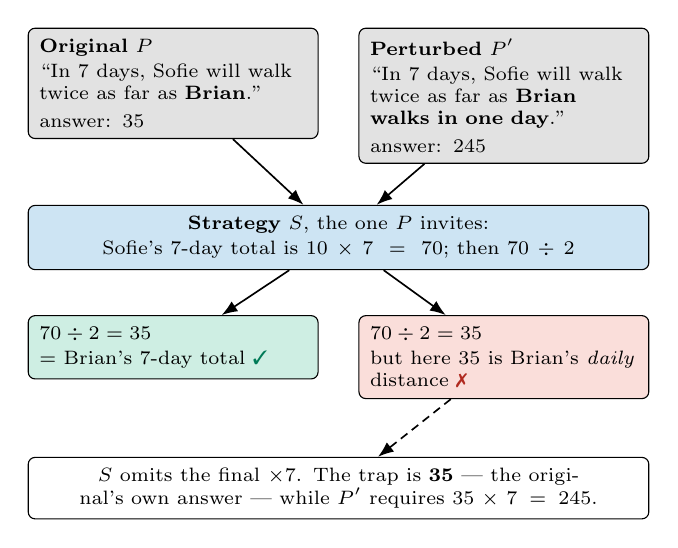
\begin{tikzpicture}[
  font=\scriptsize,
  base/.style={draw, rounded corners=2.5pt, align=left, inner sep=4pt,
               text width=34mm, anchor=north},
  wide/.style={base, text width=76mm, align=center},
  prob/.style={base, fill=cshared},
  strat/.style={wide, fill=ccode},
  good/.style={base, fill=cout},
  bad/.style={base, fill=ctrap},
  note/.style={wide, fill=white},
  ar/.style={-{Latex[length=2mm]}, semithick},
]
\node[prob] (pl) at (-2.1,0)
  {\textbf{Original $P$}\\[1pt]
   ``In 7 days, Sofie will walk twice as far as \textbf{Brian}.''\\[2pt]
   answer: $35$};
\node[prob] (pr) at (2.1,0)
  {\textbf{Perturbed $P'$}\\[1pt]
   ``In 7 days, Sofie will walk twice as far as \textbf{Brian walks in one
   day}.''\\[2pt]
   answer: $245$};

\node[strat] (s) at (0,-2.25)
  {\textbf{Strategy $S$}, the one $P$ invites:\\[1pt]
   Sofie's 7-day total is $10 \times 7 = 70$; then $70 \div 2$};

\node[good] (tl) at (-2.1,-3.65)
  {$70 \div 2 = 35$\\[1pt]
   $=$ Brian's 7-day total~\yes};
\node[bad] (tr) at (2.1,-3.65)
  {$70 \div 2 = 35$\\[1pt]
   but here $35$ is Brian's \emph{daily} distance~\no};

\node[note] (cc) at (0,-5.45)
  {$S$ omits the final $\times 7$. The trap is $\mathbf{35}$ --- the original's
   own answer --- while $P'$ requires $35 \times 7 = 245$.};

\draw[ar] (pl) -- (s);
\draw[ar] (pr) -- (s);
\draw[ar] (s) -- (tl);
\draw[ar] (s) -- (tr);
\draw[ar, densely dashed] (tr) -- (cc);
\end{tikzpicture}
\end{document}
